\documentclass{beamer}
\usetheme{Hannover}
\setbeamersize{sidebar width left=0pt}
\usepackage[T1, T2A]{fontenc}
\usepackage[utf8]{inputenc}
\usepackage[russian]{babel}
\usepackage{hyperref}
\usepackage{graphicx}
\graphicspath{ {../Images/} }

\author{Григорий Матюхин}
\date{\today}
\title{Лабораторная работа \textnumero9.}
\subtitle{Управление \texttt{SELinux}}

\begin{document}
\begin{frame}[plain]
	\titlepage
\end{frame}
\section{Цель работы}
\begin{frame}[plain]
	\frametitle{Цель работы}
	Получить навыки работы с контекстом безопасности и политиками \texttt{SELinux}.
\end{frame}

\subsection{Управление режимами SELinux}
\begin{itemize}
	\begin{frame}[plain]
		\frametitle{Управление режимами SELinux}
		\item Просмотрите текущую информацию о состоянии \texttt{SELinux}:
		\\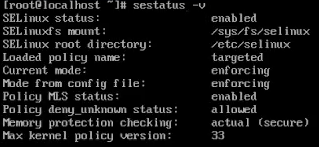
\includegraphics{1.png}
	\end{frame}
	\begin{frame}[plain]
		\item Посмотрите, в каком режиме работает \texttt{SELinux}:
		\\
\includegraphics{2.png}
	\end{frame}
	\begin{frame}[plain]
		\item Измените режим работы \texttt{SELinux} на разрешающий (\texttt{Permissive}):
		\\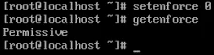
\includegraphics{3.png}
	\end{frame}
	\begin{frame}[plain]
		\item В файле \texttt{/etc/sysconfig/selinux} с помощью редактора установите \texttt{SELINUX=disabled}. Перезагрузите систему.
		\\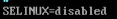
\includegraphics{4.png}
	\end{frame}
	\begin{frame}[plain]
		\item После перезагрузки запустите терминал и получите полномочия администратора.
		\item Посмотрите статус \texttt{SELinux}:
		\\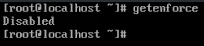
\includegraphics{5.png}
	\end{frame}
	\begin{frame}[plain]
		\item Попробуйте переключить режим работы \texttt{SELinux}:
		\\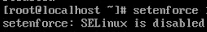
\includegraphics{6.png}
	\end{frame}
	\begin{frame}[plain]
		\item Откройте файл \texttt{/etc/sysconfig/selinux} с помощью редактора и установите \texttt{SELINUX=enforcing}. Перезагрузите систему.
		\\
\includegraphics{7.png}
	\end{frame}
	\begin{frame}[plain]
		\item После перезагрузки в терминале с полномочиями администратора просмотрите текущую информацию о состоянии \texttt{SELinux}. Убедитесь, что система работает в принудительном режиме (\texttt{enforcing}) использования \texttt{SELinux}.
		\\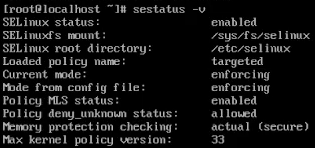
\includegraphics{8.png}
	\end{frame}
\end{itemize}

\subsection{Использование restorecon для восстановления контекста безопасности}
\begin{itemize}
	\begin{frame}[plain]
		\frametitle{Использование restorecon для восстановления контекста безопасности}
		\item Посмотрите контекст безопасности файла \texttt{/etc/hosts}:
		\\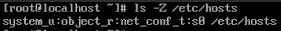
\includegraphics{9.png}
	\end{frame}
	\begin{frame}[plain]
		\item Скопируйте файл \texttt{/etc/hosts} в домашний каталог. Проверьте контекст файла \texttt{~/hosts}:
		\\
\includegraphics{10.png}
	\end{frame}
	\begin{frame}[plain]
		\item Попытайтесь перезаписать существующий файл \texttt{hosts} из домашнего каталога в каталог \texttt{/etc}:
		\item Убедитесь, что тип контекста по-прежнему установлен на \texttt{admin\_home\_t}:
		\\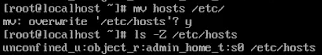
\includegraphics{11.png}
	\end{frame}
	\begin{frame}[plain]
		\item Исправьте контекст безопасности:
		\item Убедитесь, что тип контекста изменился:
		\\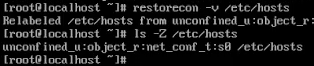
\includegraphics{12.png}
	\end{frame}
	\begin{frame}[plain]
		\item Для массового исправления контекста безопасности на файловой системе введите \texttt{touch /.autorelabel} и перезагрузите систему. Во время перезапуска не забудьте нажать клавишу \texttt{Esc} на клавиатуре, чтобы вы видели загрузочные сообщения. Вы увидите, что файловая система автоматически перемаркирована.
		\\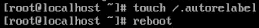
\includegraphics{13.png}
		\\
\includegraphics{14.png}
	\end{frame}
\end{itemize}

\subsection{Настройка контекста безопасности для нестандартного расположения файлов веб-сервера}
\begin{itemize}
	\begin{frame}[plain]
		\frametitle{Настройка контекста безопасности для нестандартного расположения файлов веб-сервера}
		\item Установите необходимое программное обеспечение:
		\\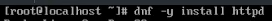
\includegraphics{15.png}
		\\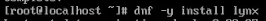
\includegraphics{15_1.png}
	\end{frame}
	\begin{frame}[plain]
		\item Создайте новое хранилище для файлов web-сервера:
		\\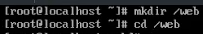
\includegraphics{16.png}
	\end{frame}
	\begin{frame}[plain]
		\item Создайте файл \texttt{index.html} в каталоге с контентом веб-сервера \texttt{Welcome to my web-server}
		\item В файле \texttt{/etc/httpd/conf/httpd.conf} проведите изченения:
		\\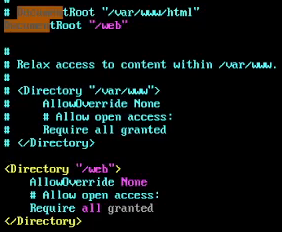
\includegraphics{17.png}
	\end{frame}
	\begin{frame}[plain]
		\item Запустите веб-сервер и службу \texttt{httpd}:
		\\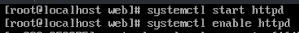
\includegraphics{18.png}
	\end{frame}
	\begin{frame}[plain]
		\item В терминале под учётной записью своего пользователя обратитесь к веб-серверу в текстовом браузере \texttt{lynx}:
		\\
\includegraphics{19.png}
	\end{frame}
	\begin{frame}[plain]
		\item В терминале с полномочиями администратора переключите \texttt{SELinux} в разрешающий режим:
		\\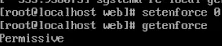
\includegraphics{20.png}
	\end{frame}
	\begin{frame}[plain]
		\item В терминале под учётной записью своего пользователя снова обратитесь к веб-серверу:
		\\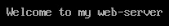
\includegraphics{21.png}
	\end{frame}
	\begin{frame}[plain]
		\item В терминале с полномочиями администратора примените новую метку контекста к \texttt{/web}:
		\\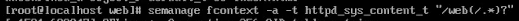
\includegraphics{22.png}
	\end{frame}
	\begin{frame}[plain]
		\item Восстановите контекст безопасности:
		\item Установите \texttt{SELinux} в режим принудительного исполнения:
		\\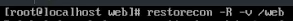
\includegraphics{23.png}
	\end{frame}
	\begin{frame}[plain]
		\item В терминале под учётной записью своего пользователя снова обратитесь к веб-серверу. Теперь вы получите доступ к своей пользовательской веб-странице.
		\\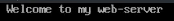
\includegraphics{24.png}
	\end{frame}
\end{itemize}

\subsection{Работа с переключателями SELinux}
\begin{itemize}
	\begin{frame}[plain]
		\frametitle{Работа с переключателями SELinux}
		\item Посмотрите список переключателей \texttt{SELinux} для службы \texttt{ftp}:
		\\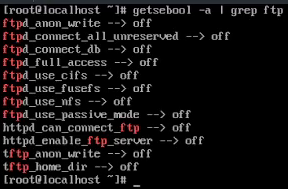
\includegraphics{25.png}
	\end{frame}
	\begin{frame}[plain]
		\item Измените постоянное значение переключателя для службы \texttt{ftpd\_anon\_write} с \texttt{off} на \texttt{on}:
		\item Посмотрите список переключателей:
		\\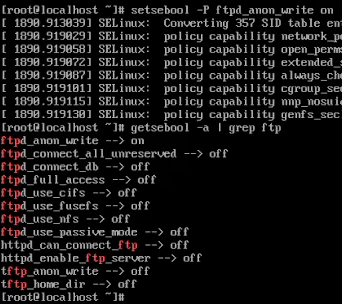
\includegraphics{26.png}
	\end{frame}
\end{itemize}

\section{Вывод}
\begin{frame}[plain]
	\frametitle{Вывод}
	В ходе выполнения данной работы я получил навыки работы с контекстом безопасности и политиками \texttt{SELinux}.
\end{frame}

\end{document}
